\documentclass{beamer}

\usepackage[utf8]{inputenc}
\usepackage[T1]{fontenc}
\usepackage{graphicx}
\usepackage{lmodern}
\usepackage{textpos}
\usepackage{pgf-umlsd}
\usepackage{listings}
\usepackage{tikz}
\usepackage{pgfplots}
\usepackage{pgfplotstable}
\usepackage[numbers,sort&compress]{natbib}
\usepackage{graphicx}
\usepackage{subcaption}

\usepgfplotslibrary{statistics}


\usepackage{t1enc}
\usepackage[utf8]{inputenc}
\usepackage{lmodern}

\usepackage[title,titletoc]{appendix}
\usepackage[section]{placeins}
\usepackage{relsize}

\usepackage[normalem]{ulem} %% Provides underlining.
\usepackage{caption} %% Provides captions.
\usepackage{mdframed} %% Provides frames around text and equations.
\usepackage{tikz-cd} %% Provides diagram drawing environment.
\usepackage{adjustbox} %% Provides additional tools to resize content.
% \usepackage[magyar]{babel} %% Provides foreign language support.

%%%%
%% Provides math related environments and directives.
\usepackage{amssymb}
\usepackage{amsthm}
\usepackage{amsmath}
\usepackage{latexsym}

\usepackage{dsfont}
\usepackage{commath}
\usepackage{bm}
\usepackage{subcaption}

%% See http://tex.stackexchange.com/questions/43835/conflict-between-amsthm-and-some-other-package
\let\proof\relax 
\let\endproof\relax

%%%%
%% Provides table environments and related directives.
\usepackage{array}
\usepackage{tabulary}
\usepackage{tabularx}
\usepackage{multirow}
\usepackage{hhline}
\usepackage{diagbox}
\usepackage{array}

%%%%
%% Provides figure environments and related directives.
\usepackage{graphicx}
\makeatletter
\def\maxwidth#1{\ifdim\Gin@nat@width>#1 #1\else\Gin@nat@width\fi}
\def\maxheight#1{\ifdim\Gin@nat@height>#1 #1\else\Gin@nat@height\fi}
\makeatother

\usepackage{fancyvrb}
\usepackage{rotating}
\frenchspacing



% Fordításhoz: pdflatex

\newcommand{\N}{\mathbb{N}}
\newcommand{\Z}{\mathbb{Z}}
\newcommand{\R}{\mathbb{R}}
\newcommand{\C}{\mathbb{C}}
\newcommand{\Hq}{\mathbb{H}}
\newcommand{\D}{\mathbb{D}}

\newcommand{\qi}{\textbf{i}}
\newcommand{\qj}{\textbf{j}}
\newcommand{\qk}{\textbf{k}}
\newcommand{\qmu}{\boldsymbol{\mu}}

\DeclareMathOperator{\rp}{Re}
\DeclareMathOperator{\ip}{Im}

\def\n{n\in\N}
\def\x{x\in\R}
\def\N{{\mathbb N}}
\def\R{{\mathbb R}}
\def\C{{\mathbb C}}
\def\Z{{\mathbb Z}}
\def\D{{\mathbb D}}
\def\B{{\mathfrak B}}
\def\T{{\mathbb T}}
\def\btheta{{\boldsymbol{\vartheta}}}
\def\bgamma{{\boldsymbol{\gamma}}}
\def\bl{{\mathbf{l}}}
\def\bk{{\mathbf{k}}}
\def\bt{{\mathbf{t}}}
\def\be{{\mathbf{e}}}


\newtheorem{definicio}{Definíció}
\newtheorem{allitas}{Állítás}
\newtheorem{kov}{Következmény}
\newtheorem{pelda}{Példa}
\newtheorem{tetel}{Tétel}


\usebackgroundtemplate{%

\includegraphics[width=\paperwidth,height=\paperheight]{background.jpg}%
}

%\setbeamercolor{title}{fg=white}
%\setbeamercolor{author}{fg=white}
%\setbeamercolor{institute}{fg=white}
%\setbeamercolor{date}{fg=white}
\setbeamercolor{frametitle}{fg=white}
%
%\title{\bf Presentation heading}
%\author{Sample Samuel}
%\institute{Eötvös Loránd University (ELTE), Budapest, Hungary}
%\date{2018}

\pgfplotsset{compat=1.16}

\begin{document}

{
\usebackgroundtemplate{
\includegraphics[width=\paperwidth]{title.jpg}}%
\begin{frame}

\color{white}{

\textbf{\Large{Color image analysis and recognition using discrete orthogonal quaternion Zernike moments}}
% \textbf{\Large{Color image analysis and recognition using quaternion Zernike moments}}

\bigskip

\Large{Zsolt Németh and Gergely Nagy}

\bigskip

\footnotesize{Eötvös Loránd University, Factulty of Informatics}
\bigskip


\large{13th Joint Conference on Mathematics and \\ Computer Science (MaCS 2020)}\\
\footnotesize{Budapest, October 1--3, 2020}
\vspace{2em}

% pozícionáljuk a dia aljához közel
\begin{textblock}{8}(0,2.5)
\footnotesize{EFOP-3.6.3-VEKOP-16-2017-00001}
\end{textblock}
}


\end{frame}
}

\section{Mathematical background}

\subsection{Image moments}
\begin{frame}{Image moments}
\vskip 3mm
The term "image moment" usually refers to some numerical descriptor of an image, computed directly from pixel intensities as a discretization of a weighted integral.\\
A well-known example: the geometric moments $$M_{pq}(I) = \int_0^1 \int_0^1 x^p y^q I(x,y)\ dx dy \approx
\sum_i \sum_j x_i^p y_j^q I(x_i,y_j).$$

\textbf{Zernike moments}: Fourier-type moments w.r.t. the Zernike function system over the unit disk $\D$.
$$Z_{n,m}(f) = \frac{n+1}{\pi}\int_0^1\int_0^{2\pi}f(r,\theta)R_{n,m}(r)e^{-\qi m\theta} r\ dr d\theta,$$ where $R_{n,m}(r)$ are an orthogonal system of \emph{radial} polynomials.
\end{frame}


\begin{frame}{Image moments for multiple channels}
\vskip 3mm
Classical approach:
\begin{itemize}
    \item Conversion of the input image to a single channel (i.e. grayscale) one.
    \item Analyze separately for each channel, merge the results later on.
\end{itemize}
An improvement for RGB over the past decade: interpret the three-channel $f : \R^2 \rightarrow \R^3$ image as a quaternion-valued function:
$$f(x,y) = \qi f_R(x,y) + \qj f_G(x,y) + \qk f_B(x,y)$$
The idea is to allow the common treatment of color channels at any point over the analysis using simple but general tools.
Examples include QFMM (Fourier--Mellin), QG-CHFM (Chebysev--Fourier), QG--PJFM (Jacobi--Fourier), \textbf{QZM (Zernike)}
\end{frame}

\subsection{Quaternion Zernike moments and invariants}
\begin{frame}{Quaternion Zernike moments}
\vskip 3mm
Generalization of Zernike functions to quaternions: $$\Phi_{n,m}(r,\theta) = R_{n,m}(r)e^{-\qmu m \theta},$$ where $\qmu$ is a pure unit quaternion (a usual choice is $\qmu = \frac{\qi + \qj + \qk}{\sqrt{3}}$).

Quaternion multiplication is generally not commutative; so we define left- and right-side moments:
$$Z^R_{n,m}(f) = \frac{n+1}{\pi}\int_0^1\int_0^{2\pi}f(r,\theta)\Phi_{n,m}(r,\theta)r\ dr d\theta,$$
$$Z^L_{n,m}(f) = \frac{n+1}{\pi}\int_0^1\int_0^{2\pi}\Phi_{n,m}(r,\theta)f(r,\theta)r\ dr d\theta.$$

Chen et al. (2012): extraction of features ($\overline{\Psi}_{n,k}^m$) from Zernike moments invariant under image translation, scaling and \emph{rotation}. 
\end{frame}

\begin{frame}{Zernike moment invariants}
\vskip 3mm
Translation: obtained by translating the origin to the centroid of the image, computed from the three channel centroids $\left(\frac{M_{10}}{M_{00}},\frac{M_{01}}{M_{00}}\right)$.

Rotation: for any $m\in\Z$ and $n,k\in\N$, the quaternions $$\Phi_{n,k}^m = Z_{n,m}^R(f)Z_{k,-m}^L(f) = -Z_{n,m}^R(f)(Z_{k,m}^R(f))^*$$ are invariant under image rotation, i.e. it is the same value for functions $f$ and $f'(r,\theta) = f(r, \theta - \alpha)$, irrespective of $\alpha$.

Scaling: certain linear combinations of Zernike moments are scaling invariant, i.e. for non-negative integers $m$ and $l$, the quaternions $$L_{m + 2l,m}^R(f) = \sum_{t=0}^l\sum_{k=t}^l\left(\sqrt{|Z_{0,0}^R(f)|}\right)^{-(m+2k+2)}c_{m,l}^{t,k}Z_{m+2t,m}^R(f)$$ are invariant under image scaling.
\end{frame}

\subsection{Discretization}
\begin{frame}{Previous approaches to discretization}
    \vskip 5mm
    \begin{figure}[tb]
        \begin{subfigure}{.30\textwidth}
        \centering
          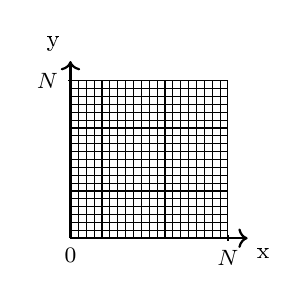
\begin{tikzpicture}
            \draw[step=0.1cm,black] (0,0) grid (2,2);
            \draw[thick,->] (0,0) -- (2.25,0) node[anchor=north west] {\footnotesize x};
            \draw[thick,->] (0,0) -- (0,2.25) node[anchor=south east] {\footnotesize y};
            \draw (2cm,1pt) -- (2cm,-1pt) node[anchor=north] {\footnotesize$N$};
            \draw (1pt,2cm) -- (-1pt,2cm) node[anchor=east] {\footnotesize$N$};
            \draw (0,0) -- (0,0) node[anchor=north] {\footnotesize$0$};
          \end{tikzpicture}
        \end{subfigure}
        \begin{subfigure}{.05\textwidth}
          \centering
          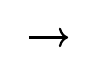
\begin{tikzpicture}
            \draw[thick,->] (0,0) -- (0.5,0);
          \end{tikzpicture}
        \end{subfigure}
        \begin{subfigure}{.30\textwidth}
          \centering
            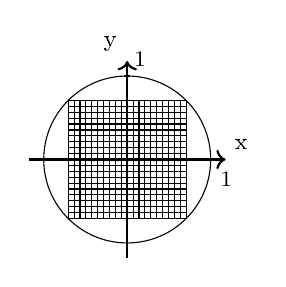
\begin{tikzpicture}
              \draw[step=0.075cm,black] (-0.75,-0.75) grid (0.75,0.75);
              \draw[thick,->] (-1.25,0) -- (1.25,0) node[anchor=south west] {\footnotesize x};
              \draw[thick,->] (0,-1.25) -- (0,1.25) node[anchor=south east] {\footnotesize y};
              \draw (0,0) circle (1.06cm);
              \draw (1.06cm,1pt) -- (1.06cm,-1pt) node[anchor=north west] {\footnotesize $1$};
              \draw (1pt,1.06cm) -- (-1pt,1.06cm) node[anchor=south west] {\footnotesize $1$};
            \end{tikzpicture}
          \end{subfigure}
      \end{figure}
      \begin{itemize}
          \item Tranformation of the image inside the unit disk: \\
                $r_{x,y} = \sqrt{(c_1x + c_2)^2 + (c_1y + c_2)^2},\ \ \ \  \theta_{x,y} = \tan^{-1}\left(\frac{c_1y + c_2}{c_1x + c_2}\right),$\\
                where $c_1 = \frac{\sqrt{2}}{N-1}$ és $c_2 = -\frac{1}{\sqrt{2}}$.
          \item Now simply use the new pixel positions for discretization:
                $$Z^R_{n,m}(f) \approx \frac{2(n+1)}{\pi(N-1)^2}\sum_{x=0}^{N-1}\sum_{y=0}^{N-1}f(x,y)\Phi_{n,m}(r_{x,y},\theta_{x,y}).$$
      \end{itemize}
\end{frame}

\begin{frame}{Novel discretization method}
\vskip 5mm

    Problem with the previous approach: no discrete orthogonality -> losing numeric precision, low robustness to noise, worse compression ratio.

    F. Schipp F. and M. Pap (2005): construction of a point system and a corresponding discrete integral for classical (complex valued) Zernike functions.

    We extended this construction for their quaternion-valued counterparts.

    Short recap: For a positive integer $N$, let $\rho_{k,N}$ denote the roots of the Legendre polynomial of degree $N$. With these, we can define the polar point system
    $$(r_{k,N}, \theta_{j,N}) = \left(\sqrt{\frac{1+\rho_{k,N}}{2}} , \frac{2\pi j}{4N} \right), \ (k=1,\ldots,N,j=1,\ldots,4N).$$
    
\end{frame}

\begin{frame}{Novel discretization method (cont.)}
    \vskip 5mm
    Now let $$\mathcal{A}_{k,N} = \int_{-1}^{1} \ell_{k,N}(x)\ dx, \ (k=1,\ldots,N),$$ denote the Christoffel numbers w.r.t the Lagrange base polynomials $\ell_{k,N}$ over $\rho_{k,N}$.
    We introduce a discrete integral w.r.t. weights $w(r_{k,N},\theta_{j,N}) = \frac{\mathcal{A}_{k,N}}{8N}$ as
    $$\frac{1}{\pi} \int_{0}^1 \int_0^{2\pi} f(r,\theta)\ d\theta dr \approx \int_{X_N} f = \sum_{k=1}^{N} \sum_{j=1}^{4N} f(r_{k,N},\theta_{j,N}) \frac{\mathcal{A}_{k,N}}{8N}.$$
    Specifically, for QZMs we obtain the approximation
    $$Z^R_{n,m}(f) \approx (n+1)\sum_{k=1}^{N}\sum_{j=1}^{4N}f(r_{k,N},\theta_{j,N})\Phi_{n,m}(r_{k,N},\theta_{j,N})\frac{\mathcal{A}_{k,N}}{8N}.$$
\end{frame}

\subsection{Discrete orthogonality}
\begin{frame}{Discrete orthogonality}
\begin{theorem}[Discrete orthogonality]
    Suppose that natural numbers $n, n' \in \N$ and integers $m, m' \in \Z$ satisfy $$\frac{n + n'}{2} + \min(|m|,|m'|) < 2N.$$
    Then we have $$(n + 1)\int_{X_N}\Phi_{n,m}\Phi_{n',m'}^* = \delta_{n,n'}\delta_{m,m'}.$$
\end{theorem}
Now, approximation of the moments can be performed without introducing further discretization errors. \\
Additionally, we also obtain the convergence of the discrete integral to the continuous one as $N\to+\infty$.
\end{frame}

\begin{frame}{Pixel transformation}

\begin{columns}
    \begin{column}{0.5\textwidth}
        \begin{figure}
            \begin{subfigure}{.48\textwidth}
                \centering
            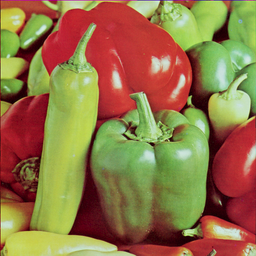
\includegraphics[width=\textwidth]{figures/pepper_color_256.png}
            \end{subfigure}
            \begin{subfigure}{.48\textwidth}
                \centering
            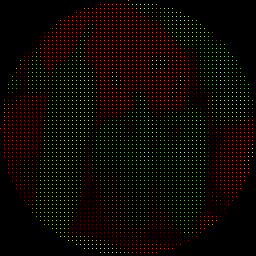
\includegraphics[width=\textwidth]{figures/pepper_square.png}
            \end{subfigure}
            \begin{subfigure}{.48\textwidth}
                \centering
            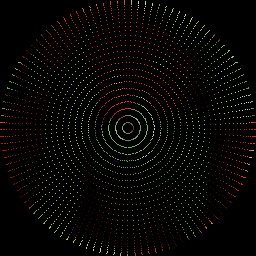
\includegraphics[width=\textwidth]{figures/pepper_bilinear.png}
            \end{subfigure}
            \begin{subfigure}{.48\textwidth}
                \centering
            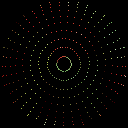
\includegraphics[width=\textwidth]{figures/pepper_integral.png}
            \end{subfigure}
        \end{figure}
    \end{column}
    \begin{column}{0.5\textwidth}
        First, we linearly transform the image to the unit disk.
        \vskip 3mm
        Second, resample the pixel data for the novel system of points:
        \begin{itemize}
            \item Linear interpolation (advised for $\approx$ the same number of points)
            \item Discrete integration locally over some neighbourhood (for a sparse system of points)
        \end{itemize}
    \end{column}
\end{columns}

\end{frame}


\section{Results}
\begin{frame}{Tests}
    \vskip 5mm
    The previous and the novel methods were compared based on the following tests:
    \begin{itemize}
    \item Invariance test
    \item Image reconstruction from the moments
    \item Recognition of transformed, noisy images
    \end{itemize}
    For these, we generated a dataset of transformed images using images from the Columbia Object Image Library and the Amsterdam Library of Object Images
    \begin{figure}[tbp]
        \begin{subfigure}{0.3\textwidth}
            \centering
        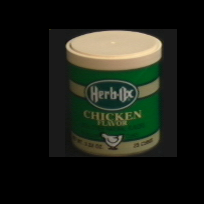
\includegraphics[width=70pt]{figures/coil_rst/26x-11y9r0s1_0.png}
        \end{subfigure}
        \begin{subfigure}{0.3\textwidth}
            \centering
        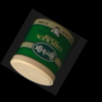
\includegraphics[width=70pt]{figures/coil_rst/26x-11y9r150s0_5.png}
        \end{subfigure}
        \begin{subfigure}{0.3\textwidth}
            \centering
        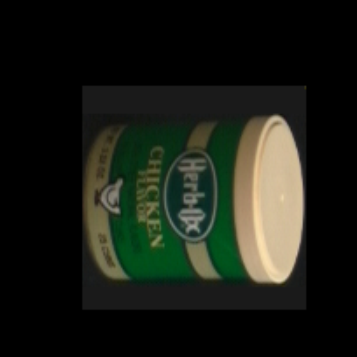
\includegraphics[width=70pt]{figures/coil_rst/26x-11y9r270s1_75.png}
        \end{subfigure}
    \end{figure}
\end{frame}

\subsection{Invariance}
\begin{frame}{Invariance}
    \vskip 10mm
The variation coefficient $\left(\frac{\sigma}{\mu}\right)$ of the modulus of low order moments over the entire transformed image set:
\begin{columns}
    \begin{column}{.5\textwidth}
        \begin{table}
            \centering
        \begin{tabular}{| c | c | } \hline
        & $\frac{\sigma}{\mu}$ \\ \hline\hline
        $|\overline{\Psi}_{1,1}^1|$ & 3.73\% \\ \hline
        $|\overline{\Psi}_{2,0}^0|$ & 0.028\% \\ \hline
        $|\overline{\Psi}_{2,2}^0|$ & 0.057\% \\ \hline
        $|\overline{\Psi}_{2,2}^2|$ & 6.87\% \\ \hline
        $|\overline{\Psi}_{3,1}^1|$ & 3.71\%  \\ \hline
        $|\overline{\Psi}_{3,3}^1|$ & 3.69\% \\ \hline
        $|\overline{\Psi}_{3,3}^3|$ & 9.40\% \\ \hline
        \end{tabular}
        \caption{Previous method}
        \end{table}
    \end{column}
    \begin{column}{.5\textwidth}
        \begin{table}
            \centering
        \begin{tabular}{| c | c | } \hline
        & $\frac{\sigma}{\mu}$ \\ \hline\hline
        $|\overline{\Psi}_{1,1}^1|$ & 3.72\% \\ \hline
        $|\overline{\Psi}_{2,0}^0|$ & 0.028\%\\ \hline
        $|\overline{\Psi}_{2,2}^0|$ & 0.056\%\\ \hline
        $|\overline{\Psi}_{2,2}^2|$ & 6.82\%\\ \hline
        $|\overline{\Psi}_{3,1}^1|$ & 3.70\%\\ \hline
        $|\overline{\Psi}_{3,3}^1|$ & 3.68\%\\ \hline
        $|\overline{\Psi}_{3,3}^3|$ & 9.32\%\\ \hline
        \end{tabular}
        \caption{Novel method}
        \end{table}
    \end{column}
\end{columns}
\end{frame}

\newcolumntype{Q}{>{\centering\arraybackslash} m{13pt} }
\newcolumntype{q}{>{\centering\arraybackslash} m{42pt} }

\subsection{Reconstruction}
\begin{frame}{Image reconstruction}
\vskip 10mm
An image can be reconstructed using a finite number of moments by the following formula: 
$$
f(x,y) \approx \sum_{n=0}^{M}\sum_{m=-n}^{n}Z_{n,m}^R(f)\Phi_{n,m}^*(r_{x,y},\theta_{x,y}).
$$
Let $f$ be the original, and $\widehat{f}$ the reconstructed image. The mean square error of the reconstruction is given by:
\begin{gather*}
    \varepsilon^2 = \frac{\displaystyle \sum_{x=1}^N\sum_{y=1}^N \left|f(x,y) - \widehat{f}(x,y)\right|^2}{\displaystyle \sum_{x=1}^N\sum_{y=1}^N \left|f(x,y)\right|^2}.
\end{gather*}
\end{frame}

\begin{frame}{Image reconstruction}
    \begin{figure}
        \centering
    \begin{tabular}{c | q q q q q }
     & Original & 50 & 100 & 150 & 250 \\ \hline\hline
    Previous & 
    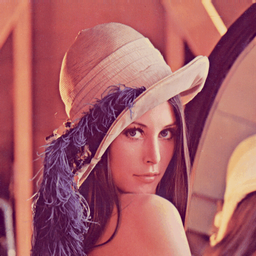
\includegraphics[width=50pt]{figures/reconstruction/lo256.png} &
    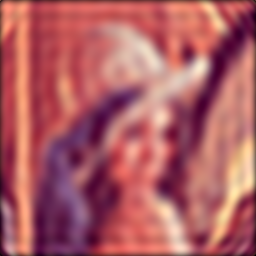
\includegraphics[width=50pt]{figures/reconstruction/lo25650.png} &
    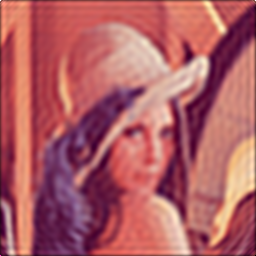
\includegraphics[width=50pt]{figures/reconstruction/lo256100.png} &
    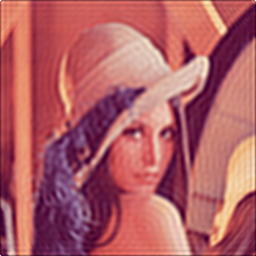
\includegraphics[width=50pt]{figures/reconstruction/lo256150.png} &
    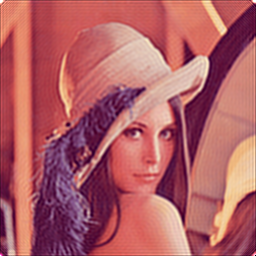
\includegraphics[width=50pt]{figures/reconstruction/lo256250.png} \\
    $\varepsilon^2$ & & 0.02659 & 0.1341 & 0.00868 & 0.00428 \\
    Novel & 
    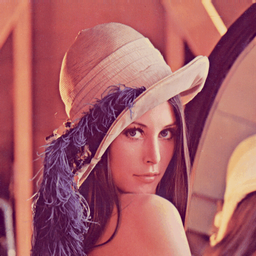
\includegraphics[width=50pt]{figures/reconstruction/lo256.png} &
    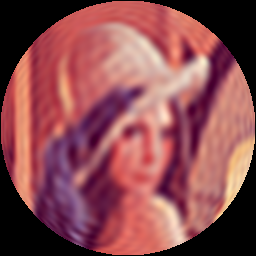
\includegraphics[width=50pt]{figures/reconstruction/ln25650.png} &
    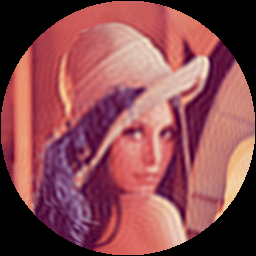
\includegraphics[width=50pt]{figures/reconstruction/ln256100.png} &
    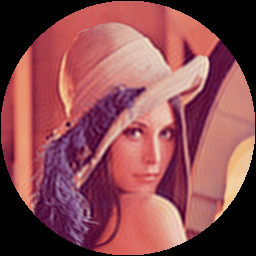
\includegraphics[width=50pt]{figures/reconstruction/ln256150.png} &
    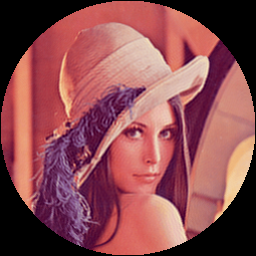
\includegraphics[width=50pt]{figures/reconstruction/ln256250.png} \\
    $\varepsilon^2$ & & 0.01611 & 0.00790 & 0.00463 & 0.00190  \\   
    \end{tabular}

    \end{figure}
\end{frame}

\subsection{Image recognition}
\begin{frame}{Image recognition}
    \vskip 5mm
Goal: correctly recognize the transformed, noisy image from the original set of images. \\
Different types of noise used for testing:
\begin{itemize}
    \item Gaussian noise
    \item Salt-and-pepper noise
\end{itemize}
Real-valued vectors are extracted from low order moments (quaternions). Classification is done by minimum Euclidean distance.
\begin{figure}[tbp]
    \begin{subfigure}{0.25\textwidth}
        \centering
    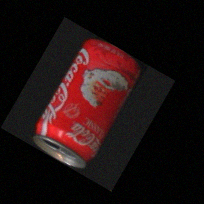
\includegraphics[width=\textwidth]{figures/noise/gauss5.png}
    \end{subfigure}
    \begin{subfigure}{0.25\textwidth}
        \centering
    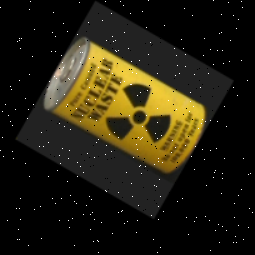
\includegraphics[width=\textwidth]{figures/noise/pepper1.png}
	\end{subfigure}
\end{figure}
\end{frame}

\begin{frame}{Image recognition - Gaussian noise}
    \vskip 1cm
    \begin{table}[tbp]
        \centering
        \begin{tabular}{|p{1.5cm}|p{2.2cm}|p{2.7cm}|p{2.5cm}|} \hline
            $\sigma$ & \textbf{Previous} (\%) & \textbf{Novel} -- "many" points (\%)& \textbf{Novel} -- "few" points (\%) \\ \hline\hline
            No noise & 99.06 & 99.15 & 98.21 \\ \hline
            1 & 98.98 & 99.49 & 98.81 \\ \hline
            2 & 98.98 & 99.74 & 98.81 \\ \hline
            3 & 98.55 & 99.83 & 98.04 \\ \hline
            5 & 95.15 & 99.49 & 94.64 \\ \hline
            7 & 95.15 & 98.72 & 91.67 \\ \hline
            9 & 76.87 & 98.47 & 89.20 \\ \hline
            40 & 52.89 & 88.52 & 51.87 \\ \hline
            50 & 48.21 & 84.10 & 45.07 \\ \hline
            60 & 41.58 & 85.80 & 39.12 \\ \hline
        \end{tabular}
    \end{table}
\end{frame}

\begin{frame}{Image recognition - Salt-and-pepper noise}
    \vskip 1cm
    \begin{table}[tbp]
        \centering
        \begin{tabular}{|p{1.5cm}|p{2.2cm}|p{2.7cm}|p{2.5cm}|} \hline
            $\sigma$ & \textbf{Previous} (\%) & \textbf{Novel} -- "many" points (\%)& \textbf{Novel} -- "few" points (\%) \\ \hline\hline
            No noise & 99.06 & 99.15 & 98.21 \\ \hline
            0.2\% & 99.66 & 99.32 & 94.98 \\ \hline
            0.4\% & 99.91 & 99.74 & 99.15 \\ \hline
            0.6\% & 99.91 & 99.91 & 99.40 \\ \hline
            1\% & 98.98 & 99.91 & 99.66 \\ \hline
            2\% & 99.66 & 93.96 & 99.74 \\ \hline
            3\% & 99.40 & 99.40 & 96.34 \\ \hline
            5\% & 97.87 & 94.90 & 97.87 \\ \hline
            10\% & 99.91 & 93.03 & 98.72 \\ \hline
            15\% & 99.91 & 93.20 & 97.87 \\ \hline
        \end{tabular}
    \end{table}
\end{frame}

\section{Summary and applications}
\begin{frame}{Applications}
\vskip 5mm
    Moment-based techniques are applicable in multiple fields, some examples:
    \begin{itemize}
    \item \textbf{Watermarking}: 
    A watermark can be placed on an image at the level of moments, thus it will be robust against different transformations and noise. The accuracy of reconstruction is important for this application.
    \item \textbf{Neural networks, machine learning}: 
    Invariant moments, extracted from the images, can be part of the input vector. A well-known issue of neural networks is their lack of robustness against noise, moments can help improve this robustness.
    \item \textbf{Face recognition and template matching}: combined with image segmentation and possibly other feature extraction methods, moment-based techniques excel at these image processing problems.
    \end{itemize}
\end{frame}

\begin{frame}{Future improvement possibilities}
    \begin{itemize}
    \item Improve existing applications based on the proposed method.
    \item Apply a similar construction to other moment methods based on various other function systems.
    \item Further generalization to 3-dimensions and application to, for example, LiDAR point clouds.
    \end{itemize}
\end{frame}

\begin{frame}{Summary}
    \begin{itemize}
    \item Construction of a discrete orthogonal point system for QZMs.
    \item Comparisons with previous methods.
        \begin{itemize}
        \item Invariance
        \item Reconstruction
        \item Image recognition
        \end{itemize}
    \item Conclusion: the novel method improves image reconstruction capability and provides robustness against various types of noise.
    \end{itemize}
\end{frame}

% this slide need not be used in the presentation, but must be
% present when you archive your talk

{
\usebackgroundtemplate{
\includegraphics[width=\paperwidth]{title.jpg}}%
\begin{frame}{}

\textbf{\huge\color{white} Thank you}

\bigskip

\textbf{\huge\color{white} for your attention!}

\end{frame}
}

\end{document}
